\documentclass[hyperref, bachelorofscience]{cgvpub}
% other document types next to bachelorofscience:
% masterofscience
% diplominf
% diplomist
% beleg

%more options (to be appended in the square brackets):
% german....... german version 
% female........ to be used for female endings in german
% bibnum....... numerical reference style
% final............ intended for the final submission
% lof.............. genereate list of figures
% lot.............. generate list of tables
% noproblem.. do not show task
% notoc......... do not generate table of contents
% twoside...... two sided layout


\author{Lucas Waclawczyk}
\title{Development of a Natural VR User Interface Using Haptic Gloves}
\birthday{26. April 1998}
\placeofbirth{Bad Langensalza}
\matno{4686687}
\betreuer{Prof. Stefan Gumhold}
\bibfiles{lib.bib}
\problem{Write down your task...}
\copyrighterklaerung{If the author used ressources from third parties (texts, images, code) he or she should state the consents of the copyright owners here or cite the given general conditions (e.g. CC/(L)GPL/BSD copyright notices)}
\acknowledgments{I'd like to thank...}
\abstracten{abstract text english}
\abstractde{ abstract text german}

\usepackage{subcaption}

\usepackage{glossaries}
\newglossary[tlg]{gloss_terms}{tld}{tdn}{Glossary}
\newglossary[slg]{gloss_acr}{sot}{stn}{Acronyms}
\makeglossaries
\loadglsentries[gloss_terms]{gloss_terms}
\loadglsentries[gloss_acr]{gloss_acr}

\newcommand{\newcite}[1]{$ ^{\text{\cite{#1}}} $}

\begin{document}
\glsaddall
	
\chapter{Introduction}


\chapter{Development}
\section{Devices and Setup}
\begin{figure}
	\begin{subfigure}{.49\linewidth}
		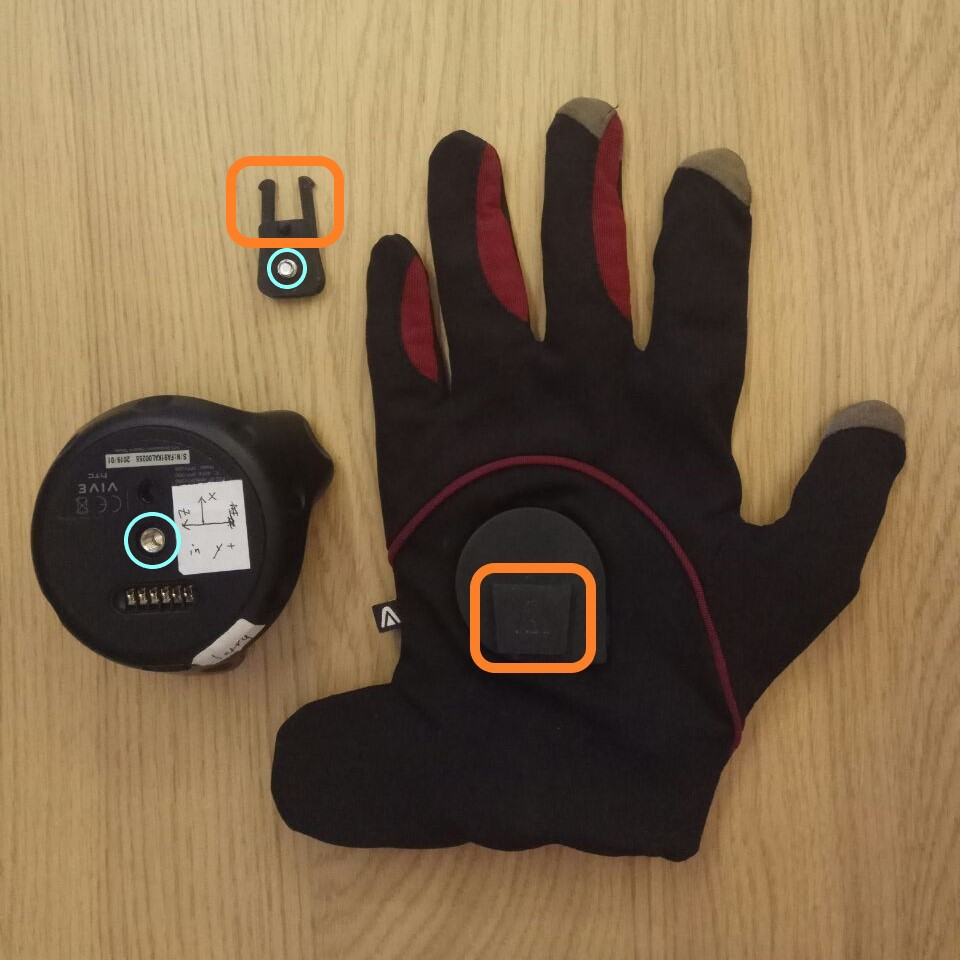
\includegraphics[width=\linewidth]{../pics/devices_uncoupled}
		\caption{Uncoupled devices, colors mark coupling point}
		\label{fig:devices:unc}
	\end{subfigure}
	\hfill
	\begin{subfigure}{.49\linewidth}
		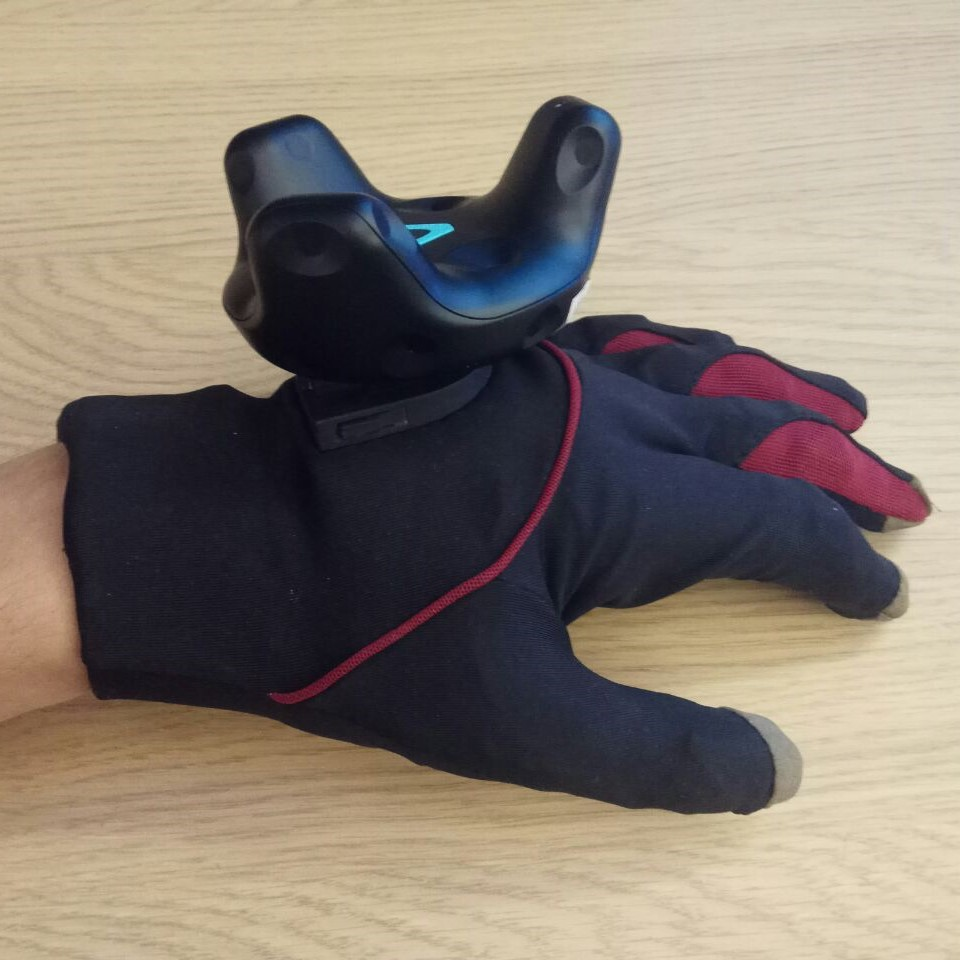
\includegraphics[width=\linewidth]{../pics/devices_coupled}
		\caption{Coupled devices on user hand}
		\label{fig:devices:cou}
	\end{subfigure}
	\caption[Devices used to track the user's hand]{Devices used to track the user's hand: Vive tracker, coupling, Avatar VR}
	\label{fig:devices}
\end{figure}

For the purpose of thesis, I used a pair of haptic gloves called Avatar VR which is a registered trademark of NeuroDigital Technologies, S. L., referred to as \acrshort{nd} hereafter. The company's details can be found at \url{neurodigital.es}.

Additionally, a Vive tracker was used to determine the user's hand position and orientation. The Avatar VR can be mechanically connected to the tracker using a coupling, that needs to be acquired separately. The named devices and the way of coupling can be seen in figure \ref{fig:devices}.

\section{Skeletal Hand Model for the Avatar VR Haptic Glove}
\subsection{Abstraction of the Human Hand Skeleton}
\begin{figure}
	\begin{subfigure}{.5\linewidth}
		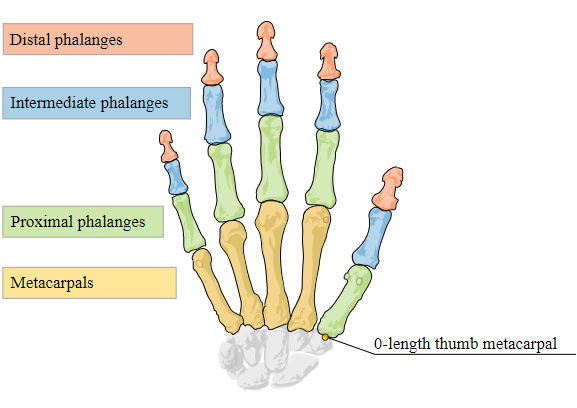
\includegraphics[width=\linewidth]{../pics/leap_anat}
		\caption{General bone structure of the human hand}
		\label{fig:hand_model:anat}
	\end{subfigure}
	\hfill
	\begin{subfigure}{.47\linewidth}
		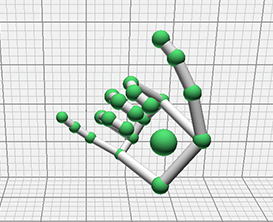
\includegraphics[width=\linewidth]{../pics/leap_example}
		\caption{Screenshot of an example hand representation in the Leap Motion API version 2.0, cropped}
		\label{fig:hand_model:leap}
	\end{subfigure}
	\caption{A model of the human hand; from \cite{leaphand}}
	\label{fig:hand_model}
\end{figure}

The human hand can be roughly divided into the parts shown in figure \ref{fig:hand_model:anat}, i.e. the \emph{\glspl{MC}}, \emph{\glspl{PPh}}, \emph{\glspl{IPh}}, and \emph{\glspl{DPh}}. A joint connecting a \gls{MC} to a \gls{PPh} is called \emph{\gls{MPJ}}, and followed by a \emph{\gls{PIJ}} and a \emph{\gls{DIJ}}.

Even though the carpals (grey in figure \ref{fig:hand_model:anat}) are physiologically quite relevant for hand movement, they stay relatively fixed compared to the other bone sets, and can thus be omitted in our simplified model. In anataomical nomenclature, the thumb is composed of \gls{PPh} and \gls{DPh} only and follows a \gls{MC}. However, this model assumes a missing \gls{MC} and existing \gls{IPh} instead which will be modelled by a 0-length \gls{MC} for uniformity reasons.

The Leap Motion API version 2.0\newcite{leaphand} uses the abstraction described above and adds
\begin{itemize}
	\item an "end" joint per finger (at the end of the \gls{DPh})
	\item a joint diagonally across the palm from the \gls{MPJ} of the index
	\item a joint in the middle of the palm
\end{itemize}

The most common representation includes cylinders for the bones and spheres for the joints. It is shown in figure \ref{fig:hand_model:leap}.

\subsection{Technology and Function of the Avatar VR}
\begin{figure}
	\centering
	\begin{subfigure}{\linewidth}
		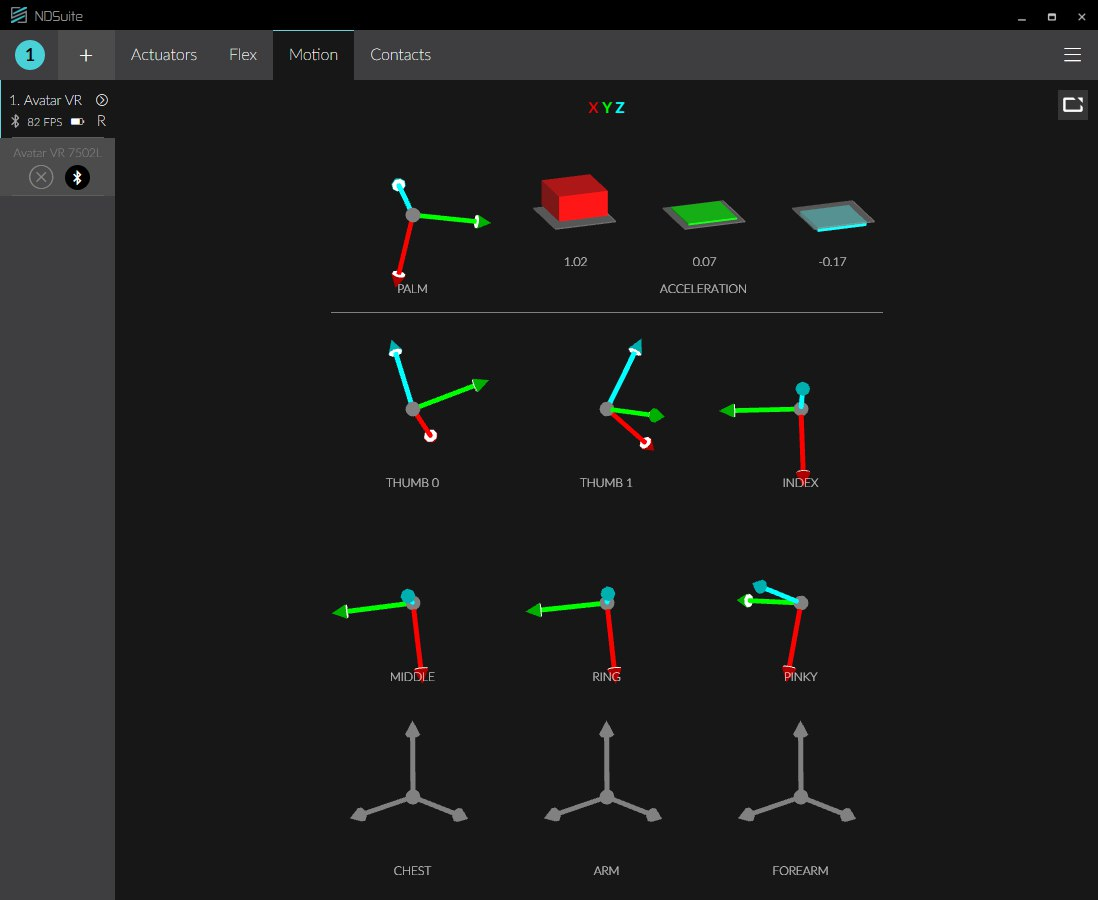
\includegraphics[width=\linewidth]{../pics/av_imus}
		\caption{"Motion" tab of ND Suite with orientations in an (optimistic) example hand pose}
		\label{fig:av_tech:imus}
	\end{subfigure}
	
	\vspace{.2cm}
	\begin{subfigure}{.45\linewidth}
		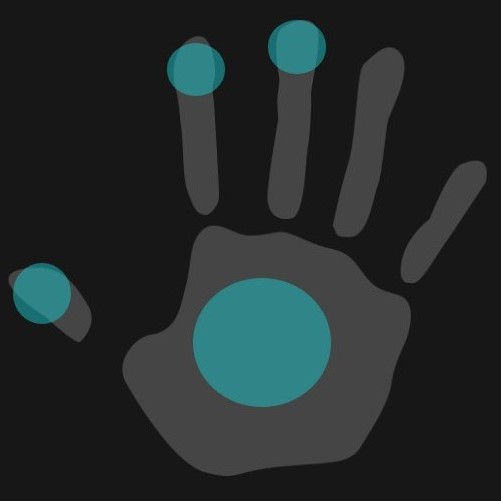
\includegraphics[width=\linewidth]{../pics/av_contacts}
		\caption{Positions of contact sensors}
		\label{fig:av_tech:contacts}
	\end{subfigure}
	\hspace{.3cm}
	\begin{subfigure}{.45\linewidth}
		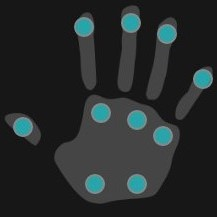
\includegraphics[width=\linewidth]{../pics/av_actu}
		\caption{Positions of actuators}
		\label{fig:av_tech:actuators}
	\end{subfigure}
	\caption{Sensors and actuators of the Avatar VR;\\screenshots of \acrshort{nd} Suite (b and c cropped)}
\end{figure}

To use the Avatar VR on a computer, one needs to download, install and run the \acrshort{nd} Suite. This program provides a background service and GUI for managing and accessing the devices. A connection can be established via Bluetooth after which all sensor data is graphically accessible from the GUI.

The Avatar VR is equipped with three kinds of sensors: 
\begin{itemize}
	\item An \emph{\acrfull{imu}} is located on the \gls{IPh} of each finger to measure its 3D rotation. The thumb is even equipped with two \acrshort{imu}s (one per phalanx) and the palm with an \acrshort{imu} that can measure both 3D orientation and 3D rotation. The "Motion" tab of \acrshort{nd} Suite shown in figure \ref{fig:av_tech:imus} depicts the resulting orientations as orthonormal bases. 
	\item At the locations marked in blue in figure \ref{fig:av_tech:contacts}, the fabric is made of an electrically conductive material. These parts are used as contact sensors (short: contacts) to determine which of the marked locations are joined.
	\item The thumb also has a flex sensor, that will not be relevant for this thesis.
\end{itemize}

Furthermore, there are actuators at the locations marked in blue in figure \ref{fig:av_tech:actuators}. These can be used for haptic feedback in a way that "[$\dots$] the brain perceives it as 'Real Touch' input", according to the producer.

\subsection{Using Data From the Avatar VR to Visualize the User's Hand}
\acrshort{nd} supplies a developer's API in the form of three files (\lstinline|NDAPI.h, NDAPI_x64.lib and NDAPI_x64.dll| or \lstinline|x86| respectively) which need to be included into the respective project in a suitable manner. A singleton of the \lstinline|NDAPI.h| can be instanstiated and used to access the data of devices connected to \acrshort{nd} Suite in the form of quaternions for rotations and booleans for pairs of contacts.

The same model used by the Leap Motion API version 2.0 will also be used here. Leap captures absolute joint positions and optimizes them for visualization. In contrast, my approach for the Avatar VR is to use a fixed resting state geometry of the user's hand (bone lengths and resting state joint positions). At the time of a \lstinline|draw()| command, the geometry is adjusted according to the data given by the glove and the Vive tracker. 

The joint position data is managed by the following struct (only most important parts included):
\begin{lstlisting}
	struct joint_positions {
		// positions of hand joints in model space
		// structure: hand_part<phalanx<position>>
		vector<vector<vec3>> positions;
		// positions linearized in hand_part major format
		// set by make_array() 
		vector<vec3> linearized;
		// correspondence of indices in linearized
		// to double indices in positions
		map<int, pair<int, int>> lin_to_anat;
				
		// rotate complete part
		void rotate(int part, quat rotation) {...}
		
		// translate complete part along neg. z-axis
		void translate_neg_z(int part, float z) {...}
		
		// translate all positions
		// used to move hand from construction origin
		// to model view location
		void translate(vec3 translation) {...}
		
		// scale all positions
		// used to realize hand size at construction origin
		void scale(float scale) {...}
		
		// generate linearized from positions
		vector<vec3> make_array() {...}
	};
\end{lstlisting}



First, the palm joints' resting positions are rotated according to the orientation given by the Vive tracker. The construction of each finger begins at the end joint of the \gls{DPh} which is translated along the negative z-axis by the hard-coded length of the \gls{DPh} and rotated by the respective quaternion (see below). The other phalanges are constructed in the same manner, before the whole finger is translated to the respective \gls{MPJ}. Finally, the whole hand is scaled to model view space and translated to the model view position of the Vive tracker.

Because the Avatar VR only returns one quaternion per finger (except for the thumb), I had to think of a way to distribute the orientation along all three phalanges 

\printglossary[type=gloss_terms]
\printglossary[type=gloss_acr]
\end{document}